\section{Result}
\label{sec:result}

\subsection{Homogeneous grid}

A homogenous grid where each node has been perturbed a small amount was used to execute the algorithm with several different choices of parameters, with a focus on the maintenance parameter, $\mu$. This is shown in fig. (\ref{fig:homogeneous}), which shows that when $\mu = 1$, i.e. the linear case, the solution that is found is the shortest path between each source and sink. When $\mu > 1$, the path chosen may not be the shortest path and there also exists a preference to share paths.

\begin{figure}
\centering
\begin{subfigure}[b]{0.48\textwidth}
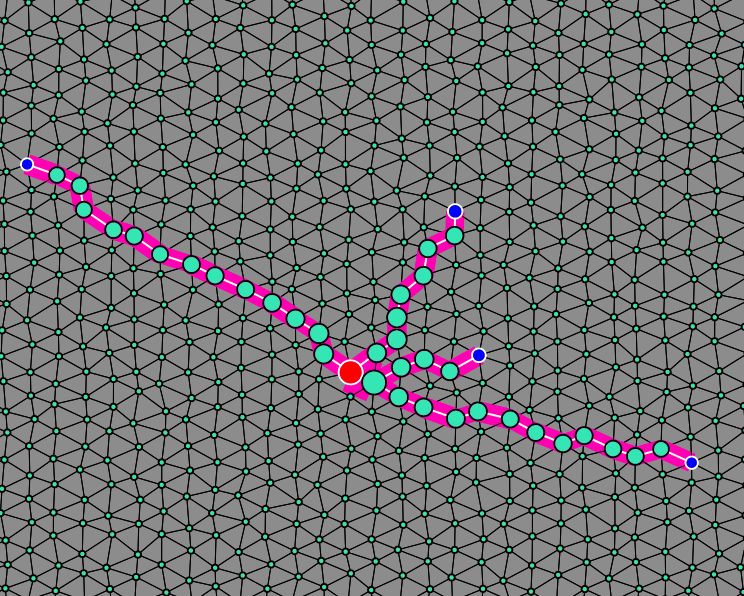
\includegraphics[width=\textwidth]{img/Lin.png}
\caption{The simulated solution when $\mu=1$. This is the shortest possible path from the source to each sink.
\\
\\}
\end{subfigure}
~
\begin{subfigure}[b]{0.48\textwidth}
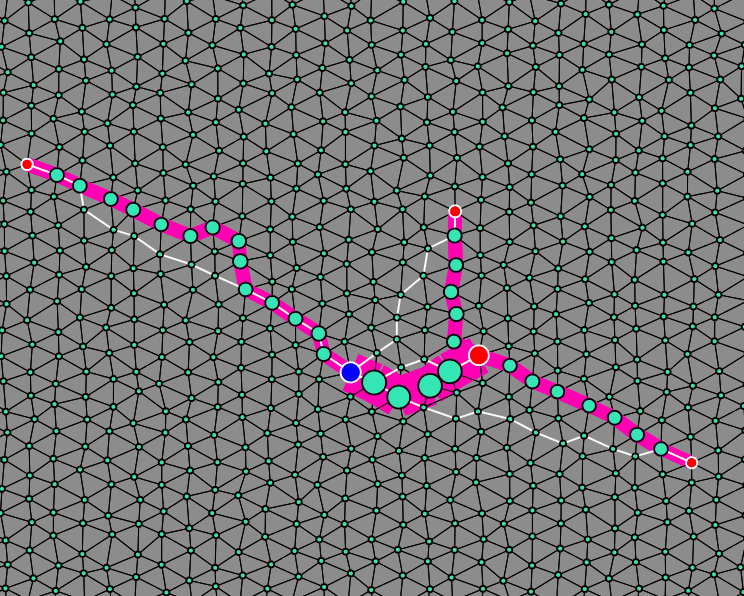
\includegraphics[width=\textwidth]{img/NonLin.png}
\caption{The simulated solution when $\mu=1.5$. This is not the shortest possible path, but rather shows a preference to take the same path as other particles, if it is not too much longer.}
\end{subfigure}
\caption{Figure shows the solutions found by the simulation on a nearly homogenous grid. The pink lines show the flow along each edge, with the thickness of the line showing the amount of flow. The shortest path from each source to each sinks has been marked with a thin white line. The parameters used are $q = 10^{-4},\lambda = 10^{-3},$ and $D_{min}=5 \cdot 10^{-2}$. Each source (red) produces 1000 particles each time unit and all sinks (blue) can together remove as many particles as are produced each time unit (evenly divided between the sinks).}
\label{fig:homogeneous}
\end{figure}

\subsection{City}

Another grid was created using road data from the city of Uppsala, Sweden.

\subsection{Parallelism}
